\documentclass[12pt,a4paper]{report}

% ------------------------------------------------------------
% Project metadata - update these fields before final submission
% ------------------------------------------------------------
\newcommand{\InstitutionName}{Indian Institute of Information technology, Allahabad}
\newcommand{\DepartmentName}{[Department Name]}
\newcommand{\SupervisorName}{[Supervisor Name]}
\newcommand{\StudentOne}{Gaurav Jaiswal}
\newcommand{\StudentTwo}{Ishan Chadha}
\newcommand{\StudentThree}{Sameer Prasad}
\newcommand{\RollOne}{IIT2023157}
\newcommand{\RollTwo}{IIT2023158}
\newcommand{\RollThree}{IIT2023134}

% ------------------------------------------------------------
% Packages
% ------------------------------------------------------------
\usepackage[utf8]{inputenc}
\usepackage[T1]{fontenc}
\usepackage{lmodern}
\usepackage[a4paper,margin=1in]{geometry}
\usepackage{graphicx}
\usepackage{amsmath,amssymb}
\usepackage{booktabs}
\usepackage{enumitem}
\usepackage[table]{xcolor}
\usepackage{caption}
\usepackage{parskip}
\usepackage{setspace}
\usepackage{titlesec}
\usepackage{fancyhdr}
\usepackage{float}
\usepackage{array}
\usepackage{tabularx}
\usepackage{multirow}
\usepackage{microtype}
\usepackage{tikz}
\usepackage{hyperref}
\usetikzlibrary{shapes.geometric, arrows.meta, positioning, shadows.blur}

% ------------------------------------------------------------
% Visual theme
% ------------------------------------------------------------
\definecolor{kbcsblue}{RGB}{19,62,110}
\definecolor{kbcsteal}{RGB}{30,126,126}
\definecolor{kbcslight}{RGB}{235,243,249}
\definecolor{kbcsgray}{RGB}{74,74,74}
\definecolor{kbcsgreen}{RGB}{52,143,80}

\graphicspath{{./}{Baseline/p4air/results/}}

\setstretch{1.25}
\linespread{1.2}
\renewcommand{\familydefault}{\sfdefault}

\hypersetup{
    colorlinks=true,
    linkcolor=kbcsblue,
    citecolor=kbcsteal,
    urlcolor=kbcsblue,
    pdftitle={KBCS Mid-Semester Report}
}

\pagestyle{fancy}
\fancyhf{}
\fancyhead[L]{Karma-Based Credit Scheduler}
\fancyhead[R]{\thepage}
\fancyfoot[C]{\small Mid-Semester Project Report}
\setlength{\headheight}{14.5pt}
\setlength{\footskip}{20pt}

\titleformat{\chapter}[display]
  {\normalfont\huge\bfseries\color{kbcsblue}}
  {\filleft\Huge\thechapter}
  {1ex}
  {\titlerule\vspace{1ex}\filright}
  [\vspace{1ex}\titlerule]

\titleformat{\section}
  {\Large\bfseries\color{kbcsteal}}
  {\thesection}{1em}{}

\titleformat{\subsection}
  {\large\bfseries\color{kbcsgray}}
  {\thesubsection}{1em}{}

% ------------------------------------------------------------
% Document
% ------------------------------------------------------------
\begin{document}

% ------------------------------------------------------------
% Title page
% ------------------------------------------------------------
\begin{titlepage}
  \centering
  \vspace*{-1cm}
  \includegraphics[width=4cm]{logo.png}\\[1.5em]
  
  {\Large \textbf{Indian Institute of Information Technology, Allahabad}}\\[0.5em]
  {\large Prayagraj, India}\\[3.5em]

  {\Huge \bfseries Karma-Based Credit Scheduler (KBCS)\\[0.4em]}
  {\LARGE \bfseries A P4-Based Fairness Mechanism for Heterogeneous TCP Flows\\[1.0em]}
  {\Large \textbf{Mid-Semester Project Report}}\\[0.8em]
  {\large Design, Baseline Evaluation, and Development Roadmap}\\[2.0em]
  {\large (6th Semester, B.Tech. IT)}\\[2em]
  \rule{0.9\textwidth}{1pt}\\[2em]

  {\large \textbf{Team Members:}}\\[1.0em]
  \begin{itemize}[label=\textbullet, leftmargin=3.2cm]
      \item \StudentOne\ (\RollOne)
      \item \StudentTwo\ (\RollTwo)
      \item \StudentThree\ (\RollThree)
  \end{itemize}

  \vfill
  \rule{0.55\textwidth}{0.4pt}\\[0.3em]
  {\small Submitted to \SupervisorName}\\[0.2em]
  {\small March 2026}
\end{titlepage}

\pagenumbering{roman}
\clearpage

% ------------------------------------------------------------
% Certificate
% ------------------------------------------------------------
\chapter*{Certificate}
\addcontentsline{toc}{chapter}{Certificate}
This is to certify that the project report entitled \textbf{``Karma-Based Credit Scheduler (KBCS): A P4-Based Fairness Mechanism for Heterogeneous TCP Flows''} submitted by \textbf{\StudentOne, \StudentTwo, and \StudentThree} is a record of bona fide work carried out under my supervision as part of the mid-semester project evaluation.

\vspace{4cm}
\begin{flushright}
  \rule{5cm}{0.4pt} \\
  \vspace{0.2cm}
  \textbf{\SupervisorName} \\
  \vspace{0.2cm}
  \DepartmentName \\
  \InstitutionName
\end{flushright}
\clearpage

% ------------------------------------------------------------
% Declaration
% ------------------------------------------------------------
\chapter*{Candidate Declaration}
\addcontentsline{toc}{chapter}{Candidate Declaration}
We, \StudentOne, \StudentTwo, and \StudentThree, hereby declare that this report is an original account of our project work on \textbf{Karma-Based Credit Scheduler (KBCS)}. The work presented here has been prepared for academic evaluation, and all external ideas, papers, and implementation references used during the project have been acknowledged in the report.

We understand that plagiarism includes:
\begin{enumerate}
    \item presenting another person's work or ideas as our own,
    \item reproducing text, code, or design without proper attribution, and
    \item using technical material from prior work without clear acknowledgment.
\end{enumerate}

We affirm that this report honestly distinguishes among completed implementation, baseline results already obtained, and advanced KBCS features that remain under development.

\vspace{2cm}
\textbf{Date:} March 2026

\vspace{1cm}
\begin{flushleft}
\StudentOne\ (\RollOne) \\
\StudentTwo\ (\RollTwo) \\
\StudentThree\ (\RollThree)
\end{flushleft}

\vspace{1cm}
\begin{flushleft}
\textbf{\DepartmentName} \\
\textbf{\InstitutionName}
\end{flushleft}
\clearpage

% ------------------------------------------------------------
% Abstract
% ------------------------------------------------------------
\chapter*{Abstract}
\addcontentsline{toc}{chapter}{Abstract}
Fair bandwidth sharing among competing TCP congestion control algorithms remains a central challenge in programmable data-plane networking. When aggressive loss-based flows such as CUBIC share a bottleneck with model-based or delay-sensitive flows such as BBR, conventional FIFO buffering often leads to queue domination, elevated latency, and throughput unfairness. This project studies that problem in a P4-programmable environment and proposes the \textbf{Karma-Based Credit Scheduler (KBCS)}, a lightweight fairness mechanism that assigns per-flow credit scores inside the switch dataplane.

The project is organized around two components. First, we implemented and evaluated \textbf{P4air} as a strong baseline in BMv2 and Mininet. P4air provides congestion-control-aware fingerprinting, queue reallocation, and action modules, and its experimental results establish the fairness-performance reference point that KBCS must match or improve. Second, we designed KBCS as a simpler alternative that tracks a decayed per-flow byte estimate, updates a bounded karma value, maps flows into behavioral classes, and ultimately aims to use priority-aware queue management to protect well-behaved traffic from aggressive flows.

At the current project stage, the repository contains a working KBCS prototype, a plain forwarding baseline, a Mininet evaluation topology, and automation scripts for comparative testing. However, the full queue-depth-aware KBCS described in the enhanced design document is not yet completely integrated. Therefore, this report deliberately separates measured baseline results from planned KBCS features and presents a realistic roadmap toward the end-semester implementation and evaluation.
\clearpage

\tableofcontents
\clearpage
\listoffigures
\clearpage
\listoftables
\clearpage
\pagenumbering{arabic}

% ------------------------------------------------------------
\chapter{Introduction and Motivation}

\section{Motivation}
Modern networks routinely carry flows governed by different TCP congestion control algorithms (CCAs). In such heterogeneous environments, bandwidth competition is not neutral: aggressive loss-based senders tend to occupy buffer space more quickly, while model-based or delay-sensitive senders back off earlier. The outcome is often unfair bandwidth distribution at the bottleneck, especially when all packets share a single FIFO queue.

This problem is particularly relevant in programmable networking, where P4-capable switches offer an opportunity to move fairness logic into the data plane. Instead of waiting for end hosts to coordinate, a switch can observe packet behavior in real time and apply per-flow scheduling, queueing, or dropping decisions before unfairness fully develops.

\section{TCP Congestion Control: A Brief Theoretical Overview}
TCP congestion control is the mechanism by which end hosts regulate their sending rates to avoid overwhelming the network. Since Jacobson's seminal work on the ``conservation of packets'' principle~\cite{jacobson88}, numerous CCA variants have been developed, each optimizing for different network conditions. These algorithms can be broadly classified into four families, as shown in Table~\ref{tab:cca_families}.

\begin{table}[H]
\centering
\caption{Taxonomy of TCP congestion control algorithm families~\cite{p4air,p4cci}}
\label{tab:cca_families}
\renewcommand{\arraystretch}{1.35}
\begin{tabularx}{\textwidth}{@{}p{2.8cm}p{3.2cm}p{3.5cm}X@{}}
\toprule
\textbf{CCA Family} & \textbf{Primary Signal} & \textbf{Representative CCAs} & \textbf{Aggressiveness} \\
\midrule
Purely Loss-Based & Packet loss & CUBIC, Reno, BIC, HighSpeed & Highest — fills buffer until loss occurs \\
Loss-Delay Hybrid & Loss + RTT increase & Illinois, YeAH, Veno, Hybla & Medium — uses delay as secondary signal \\
Delay-Based & RTT increase & Vegas, LoLa & Lowest — backs off at first sign of queuing \\
Model-Based & BDP estimation & BBR & Variable — periodic bandwidth probing \\
\bottomrule
\end{tabularx}
\end{table}

\subsection{The Bufferbloat Problem}
When loss-based algorithms such as CUBIC share a bottleneck with delay-sensitive algorithms such as BBR or Vegas, a fundamental conflict arises. CUBIC's AIMD (Additive Increase, Multiplicative Decrease) strategy deliberately fills the buffer to detect the link capacity — it \textit{requires} packet loss as a congestion signal. In contrast, BBR estimates the bottleneck bandwidth and round-trip propagation time to construct a model of the network path, aiming to keep exactly one Bandwidth-Delay Product (BDP) of data in flight~\cite{hint}. Figure~\ref{fig:cca_competition} illustrates this buffer competition.

\begin{figure}[H]
\centering
\resizebox{0.92\textwidth}{!}{%
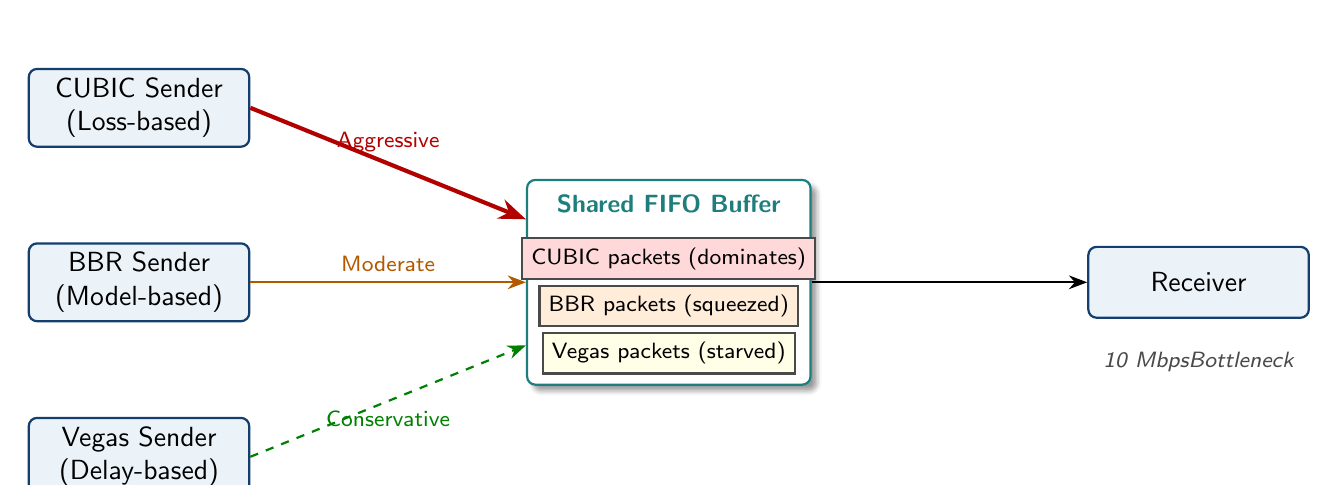
\begin{tikzpicture}[
  node distance=0.8cm and 1.8cm,
  host/.style={rectangle, draw=kbcsblue, fill=kbcslight, thick, minimum width=2.8cm, minimum height=0.9cm, align=center, rounded corners=3pt},
  switch/.style={rectangle, draw=kbcsteal, fill=white, thick, minimum width=3.6cm, minimum height=2.6cm, align=center, rounded corners=3pt, blur shadow},
  queue/.style={rectangle, draw=kbcsgray, thick, minimum width=2.6cm, minimum height=0.5cm, align=center, font=\footnotesize},
  arrow/.style={->, >=Stealth, thick},
  label/.style={font=\footnotesize\itshape, text=kbcsgray}
]

\node[host] (cubic) {CUBIC Sender\\(Loss-based)};
\node[host, below=1.2cm of cubic] (bbr) {BBR Sender\\(Model-based)};
\node[host, below=1.2cm of bbr] (vegas) {Vegas Sender\\(Delay-based)};

\node[switch, right=3.5cm of bbr] (sw) {};
\node[font=\bfseries\small, text=kbcsteal] at ([yshift=1.0cm]sw.center) {Shared FIFO Buffer};

\node[queue, fill=red!15] at ([yshift=0.3cm]sw.center) {CUBIC packets (dominates)};
\node[queue, fill=orange!15] at ([yshift=-0.3cm]sw.center) {BBR packets (squeezed)};
\node[queue, fill=yellow!10] at ([yshift=-0.9cm]sw.center) {Vegas packets (starved)};

\node[host, right=3.5cm of sw] (recv) {Receiver};
\node[label, below=0.3cm of recv] {10 Mbps\\Bottleneck};

\draw[arrow, red!70!black, line width=1.5pt] (cubic.east) -- ([yshift=0.8cm]sw.west) node[midway, above, font=\footnotesize] {Aggressive};
\draw[arrow, orange!70!black] (bbr.east) -- (sw.west) node[midway, above, font=\footnotesize] {Moderate};
\draw[arrow, green!50!black, dashed] (vegas.east) -- ([yshift=-0.8cm]sw.west) node[midway, below, font=\footnotesize] {Conservative};
\draw[arrow] (sw.east) -- (recv.west);

\end{tikzpicture}%
}
\caption{Buffer competition when heterogeneous CCAs share a FIFO bottleneck queue. Loss-based flows like CUBIC dominate the buffer, squeezing delay-sensitive flows.}
\label{fig:cca_competition}
\end{figure}

When these algorithms share a single FIFO queue, CUBIC fills the buffer completely, causing BBR to observe inflated RTTs and Vegas to back off entirely. The result is that CUBIC receives a disproportionately large share of the bandwidth, a phenomenon well-documented in the literature~\cite{p4air, ccaaware, buffermgmt}.

\subsection{The Role of Active Queue Management}
Active Queue Management (AQM) mechanisms attempt to signal congestion to end hosts \textit{before} the buffer overflows. Classical AQM algorithms such as RED (Random Early Detection) and CoDel (Controlled Delay) use probabilistic dropping or sojourn-time thresholds to manage queue occupancy. However, these mechanisms are flow-agnostic — they apply the same policy to all packets regardless of the sender's behavior. As a result, they cannot differentiate between an aggressive CUBIC flow that \textit{caused} the congestion and a well-behaved Vegas flow that is merely a victim of it~\cite{ccaaware, pfq}.

\section{Programmable Data Planes and P4}
The emergence of the P4 programming language~\cite{p4lang} has opened a new avenue for addressing fairness at the network layer. P4 enables protocol-independent packet processing in which the switch pipeline — parser, match-action tables, and deparser — is defined by the network operator rather than fixed by the silicon vendor.

In the \textbf{v1model} architecture used by BMv2 (Behavioral Model version 2), the pipeline consists of six programmable blocks: parser, verify checksum, ingress control, egress control, compute checksum, and deparser. This architecture provides access to stateful elements such as \textbf{registers}, \textbf{counters}, and \textbf{meters}, enabling per-flow state tracking at line rate~\cite{p4cci, p5}.

For this project, the key insight is that P4 registers can store per-flow behavioral state (e.g., byte counts, karma values) that persists across packets, allowing the switch to build a flow-level behavioral profile and apply differentiated treatment \textit{within the data plane itself}, without control-plane intervention on a per-packet basis.

\section{Project Context}
Our project investigates the TCP fairness problem through two complementary systems:
\begin{itemize}
    \item \textbf{P4air}~\cite{p4air}, an existing state-of-the-art baseline that performs CCA fingerprinting directly in the P4 data plane and enforces fairness through queue reallocation and corrective actions.
    \item \textbf{KBCS}, our proposed karma-based scheduler that aims to provide equivalent or superior fairness with simpler dataplane logic and improved robustness in software-emulated environments.
\end{itemize}

The project uses BMv2, Mininet, and P4\_16 to construct a controlled dumbbell topology in which multiple senders compete over a 10 Mbps bottleneck. Figure~\ref{fig:dumbbell_topology} shows the experimental topology used throughout this project.

\begin{figure}[H]
\centering
\resizebox{0.85\textwidth}{!}{%
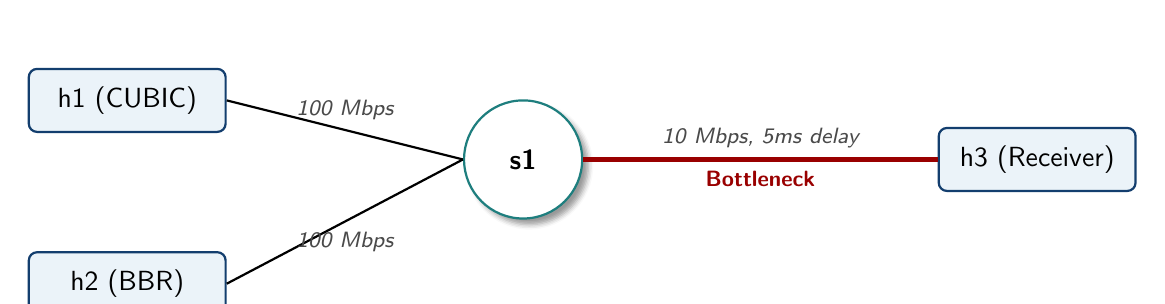
\begin{tikzpicture}[
  host/.style={rectangle, draw=kbcsblue, fill=kbcslight, thick, minimum width=2.5cm, minimum height=0.8cm, align=center, rounded corners=3pt},
  sw/.style={circle, draw=kbcsteal, fill=white, thick, minimum size=1.5cm, align=center, font=\bfseries, blur shadow},
  label/.style={font=\footnotesize\itshape, text=kbcsgray},
  arrow/.style={-, thick}
]

\node[host] (h1) {h1 (CUBIC)};
\node[host, below=1.5cm of h1] (h2) {h2 (BBR)};
\node[sw, right=3cm of h1, yshift=-0.75cm] (s1) {s1};
\node[host, right=4.5cm of s1] (h3) {h3 (Receiver)};

\draw[arrow] (h1.east) -- (s1.west) node[midway, above, label] {100 Mbps};
\draw[arrow] (h2.east) -- (s1.west) node[midway, below, label] {100 Mbps};
\draw[arrow, red!60!black, line width=1.5pt] (s1.east) -- (h3.west) node[midway, above, label] {10 Mbps, 5ms delay} node[midway, below, font=\footnotesize\bfseries, text=red!60!black] {Bottleneck};

\end{tikzpicture}%
}
\caption{Dumbbell topology used in the KBCS experimental environment. The 10:1 bandwidth ratio at the bottleneck forces CCA competition.}
\label{fig:dumbbell_topology}
\end{figure}

\section{Why KBCS is Needed}
The repository already shows an important design tension. Sophisticated systems such as P4air can achieve strong fairness under the right conditions, but they rely on detailed flow fingerprinting including RTT estimation, BDP calculation, and queue-growth streak tracking. In software-emulated environments, that complexity can introduce instability and high variance — as our baseline experiments demonstrate, P4air's throughput standard deviation reaches $\pm 1.61$ Mbps in the 30-run test compared to $\pm 0.27$ Mbps for simple FIFO~\cite{repo}.

KBCS is motivated by the idea that a smaller, behavior-based scheduler may achieve competitive fairness with lower implementation complexity and fewer timing assumptions. This aligns with the practical observation from several recent works~\cite{buffermgmt, ccaaware} that simpler queue management policies can be more robust under software emulation constraints.

% ------------------------------------------------------------
\chapter{Problem Statement and Objectives}

\section{Problem Statement}
The central problem addressed in this project is:

\textit{How can a P4-programmable switch improve fairness among heterogeneous TCP flows at a shared bottleneck without modifying the end hosts, while remaining implementable under the practical constraints of BMv2 and hardware-oriented P4 dataplanes?}

More specifically, we focus on competition between CUBIC and BBR style flows and study how queue management decisions at the switch can reduce domination by aggressive senders.

\section{Project Objectives}
The project has the following concrete objectives:
\begin{itemize}
    \item implement and validate P4air as a fairness baseline in BMv2 and Mininet,
    \item design KBCS as a simpler switch-resident fairness mechanism based on per-flow credit scores,
    \item build a reusable experimental topology for baseline and KBCS comparison,
    \item evaluate fairness using Jain's Fairness Index and throughput-based metrics, and
    \item complete a queue-aware KBCS implementation that can be compared directly against the baseline systems.
\end{itemize}

\section{Design Philosophy}
KBCS follows a ``fast penalty, slow recovery'' strategy. A flow that persistently exhibits aggressive behavior should be demoted quickly, while a previously penalized flow should regain trust gradually. This asymmetry is important because it avoids oscillation and stabilizes queue behavior under repeated congestion.

% ------------------------------------------------------------
\chapter{Background and Related Work}

This chapter presents a comprehensive review of the literature that informed the design of KBCS. The reviewed works span four principal areas: (i) CCA-aware data plane systems, (ii) P4-based buffer and queue management, (iii) fair queueing and proactive scheduling, and (iv) in-band network telemetry for congestion feedback. A taxonomic summary is provided in Table~\ref{tab:literature_taxonomy} before individual works are discussed in detail.

\begin{table}[H]
\centering
\caption{Taxonomy of reviewed literature by research focus area}
\label{tab:literature_taxonomy}
\renewcommand{\arraystretch}{1.3}
\begin{tabularx}{\textwidth}{@{}p{3.8cm}p{3.2cm}X@{}}
\toprule
\textbf{Focus Area} & \textbf{Papers} & \textbf{Core Contribution} \\
\midrule
CCA-aware data plane fairness & P4air~\cite{p4air}, P4CCI~\cite{p4cci}, Real-Time CCA ID~\cite{realtimecca} & In-switch identification and differentiated treatment of CCA families \\
Buffer and queue management & CCA-aware QM~\cite{ccaaware}, P4 Buffer Mgmt~\cite{buffermgmt} & Programmable queue policies for throughput fairness \\
Fair queueing schemes & PFQ~\cite{pfq} & Proactive fairness with high utilization guarantees \\
In-band network telemetry & HINT~\cite{hint} & P4-driven telemetry for congestion feedback \\
Multi-agent congestion control & MARL-CC~\cite{marlcc} & Deep reinforcement learning for cooperative fairness \\
P4 traffic engineering & P5~\cite{p5}, P4-NEON~\cite{p4neon} & Event-driven and SDN-based P4 policy frameworks \\
\bottomrule
\end{tabularx}
\end{table}

% --- Section: CCA-aware systems ---
\section{CCA-Aware Data Plane Systems}

\subsection{P4air: Increasing Fairness among Competing CCAs}
The strongest baseline in this project is \textbf{P4air}, proposed by Turkovic and Kuipers~\cite{p4air}. P4air implements a three-module pipeline directly in the P4 data plane:

\begin{enumerate}
    \item \textbf{Fingerprinting Module}: classifies each TCP flow into one of four CCA groups — \textit{purely loss-based} (e.g., CUBIC, Reno), \textit{loss-delay hybrid} (e.g., Illinois, YeAH), \textit{delay-based} (e.g., Vegas), and \textit{model-based} (e.g., BBR). Classification is performed by tracking per-RTT packet counts, queue-depth growth streaks, and periodic bandwidth probing patterns.
    \item \textbf{Reallocation Module}: dynamically adjusts queue boundaries among the four groups. Groups with more active flows receive proportionally more hardware queues from a pool of 8 priority queues ($Q_0$--$Q_7$), with $Q_0$ and $Q_1$ reserved for short (``ant'' and ``mice'') flows.
    \item \textbf{Apply Actions Module}: enforces differentiated penalties when a flow exceeds its estimated fair share (BDP threshold): loss-based flows are \textit{dropped}, delay-based flows are \textit{recirculated} (delayed), and model-based (BBR) flows have their TCP receiver window \textit{halved}.
\end{enumerate}

The flow lifecycle in P4air follows a progressive classification path:
\[
\text{New flow} \rightarrow \text{Ant} \rightarrow \text{Mice} \xrightarrow{\text{slow-start ends}} \text{Delay-Based} \xrightarrow{m_{LD} \text{ RTTs}} \text{Loss-Delay} \xrightarrow{m_{PL} \text{ RTTs}} \text{Purely Loss}
\]
with a model-based branch triggered when periodic bandwidth probing is detected ($m_M$ consecutive patterns). The default thresholds are $m_{LD}=4$, $m_{PL}=12$, and $m_M=4$ RTT intervals~\cite{p4air}.

P4air reports fairness indices of approximately $0.87$--$0.96$ across various CCA mixtures (vs. $0.18$--$0.49$ without intervention) while maintaining link utilization above $90\%$. However, as our own evaluation in Chapter~7 shows, this performance degrades significantly in software-emulated environments (BMv2) due to timing jitter and recirculation overhead.

P4air is the most directly relevant prior work because it represents the strongest known CCA-aware fairness baseline. Any improvement claimed by KBCS must be validated against P4air, not merely against FIFO or static queueing.

\subsection{P4CCI: Online TCP CCA Identification}
P4CCI~\cite{p4cci} focuses exclusively on the CCA classification problem. It proposes a lightweight P4-based mechanism for \textit{real-time} identification of which congestion control algorithm a given flow is running, without relying on deep packet inspection or payload analysis.

P4CCI's approach involves per-flow tracking of sending rate patterns, loss response behavior, and delay sensitivity using P4 registers. By observing how a flow reacts to network events (e.g., does it halve its rate on loss, or does it probe bandwidth periodically?), the switch can assign flows to CCA categories with high accuracy. The work demonstrates that P4's stateful processing capabilities are sufficient for behavioral fingerprinting of TCP flows at the data plane.

The relevance to KBCS is twofold. First, P4CCI validates that per-flow behavioral profiling is feasible within P4 hardware constraints. Second, KBCS adopts a philosophically similar but deliberately simpler approach: instead of identifying the \textit{exact} CCA, KBCS observes whether a flow is \textit{behaving aggressively} (high sending rate relative to its fair share) and assigns consequences accordingly through karma scores.

\subsection{Real-Time CCA Identification with P4 Switches}
This work~\cite{realtimecca} extends the CCA identification paradigm by focusing on real-time classification accuracy and low detection latency. It demonstrates that P4 programmable switches can classify TCP flows into CCA families within a few RTT intervals, enabling rapid response to emerging unfairness.

The key distinction from P4CCI is the emphasis on online classification speed versus offline accuracy. For KBCS, this work reinforces the importance of \textit{fast reaction time} — a principle embodied in our ``fast penalty, slow recovery'' strategy where karma degradation is swift ($-5$ per aggressive packet) while recovery is gradual ($+1$ per well-behaved packet).

% --- Section: Buffer and Queue Management ---
\section{P4-Based Buffer and Queue Management}

\subsection{CCA-Aware Queue Management}
This work~\cite{ccaaware} proposes using CCA awareness to separate aggressive and sensitive traffic into different queues at the switch. Rather than applying the same AQM policy to all traffic, the authors argue that queue management decisions should be differentiated based on the sender's congestion control behavior.

The key insight is that applying a single DROP or ECN policy uniformly to all flows is fundamentally unfair: a loss-based flow like CUBIC \textit{interprets} a drop as a congestion signal and reduces its window, which is the intended behavior. But a delay-based flow like Vegas may never recover its fair share once it has been penalized, because it interprets the resulting RTT increase as a sign to back off further~\cite{ccaaware}.

This directly motivates the KBCS design principle of \textbf{differentiated treatment}: green-class flows (high karma) should be protected from the same AQM actions that are applied to red-class flows (low karma). KBCS achieves this through priority queue mapping rather than per-CCA policies, making it simpler to implement while achieving a similar protective effect.

\subsection{P4-Based Buffer Management for Throughput Fairness}
This paper~\cite{buffermgmt} proposes a P4-based buffer management method that improves throughput fairness when different CCAs contend for the same bottleneck. The approach uses programmable queue control within the P4 data plane to enforce per-flow buffer occupancy limits.

The authors demonstrate that by monitoring per-flow buffer usage through P4 registers and applying selective dropping when a single flow occupies more than its fair share of the buffer, throughput fairness can be significantly improved without requiring CCA identification. This ``buffer-occupancy-aware'' approach is conceptually related to KBCS's decayed byte tracking, which similarly measures per-flow sending intensity without attempting full CCA classification.

The reported results show that the method improves Jain's Fairness Index from approximately $0.5$ to above $0.9$ in mixed CUBIC/BBR scenarios, while maintaining total throughput above $90\%$ of link capacity~\cite{buffermgmt}. These numbers provide an additional performance reference point for our KBCS evaluation.

% --- Section: Fair Queueing ---
\section{Fair Queueing and Proactive Scheduling}

\subsection{PFQ: Proactive Fair Queueing}
PFQ (Proactive Fair Queueing)~\cite{pfq} addresses the fairness-utilization tradeoff in data center networks. Unlike reactive approaches that penalize aggressive flows \textit{after} unfairness has developed, PFQ proactively distributes traffic across queues to \textit{prevent} unfairness from occurring.

PFQ's key contribution is demonstrating that fairness and high utilization are not inherently conflicting objectives. By carefully designing queue weights and scheduling policies, a switch can maintain near-perfect fairness ($J > 0.95$) while achieving utilization above $95\%$~\cite{pfq}. This finding is directly relevant to KBCS because it validates that our queue-mapping approach (green $\rightarrow$ high-priority, yellow $\rightarrow$ medium, red $\rightarrow$ low-priority) can achieve fairness without sacrificing throughput, provided the queue weights are properly tuned.

The PFQ framework also highlights the importance of \textbf{rapid state convergence}: the queueing system must adapt quickly when flow conditions change. KBCS's asymmetric karma update ($-5/+1$) is designed precisely to achieve fast convergence toward the correct behavioral classification while avoiding oscillation.

% --- Section: Telemetry ---
\section{In-Band Network Telemetry for Congestion Control}

\subsection{HINT: P4-Driven In-Band Network Telemetry}
HINT~\cite{hint} explores the use of P4-driven In-Band Network Telemetry (INT) to support congestion control decisions. INT allows switches to embed network state information (e.g., queue depth, link utilization, processing latency) directly into packet headers, providing end hosts with fine-grained visibility into network conditions.

HINT demonstrates that INT-enriched feedback can enable significantly better congestion control decisions compared to traditional implicit signals (loss, delay). For instance, a sender equipped with INT data can distinguish between different types of congestion — whether a buffer is filling due to a microburstiness or sustained overload — and respond appropriately~\cite{hint}.

For KBCS, HINT suggests an important future extension: the karma update logic could incorporate \texttt{standard\_metadata.enq\_qdepth} (queue depth at enqueue time) as an additional input signal. The enhanced KBCS design document already specifies queue-depth-aware decision making as a planned feature, and HINT validates that this approach can yield substantial improvements in congestion response quality.

% --- Section: Other Related Work ---
\section{Other Related Work}

\subsection{Multi-Agent Reinforcement Learning for Congestion Control}
The work by the authors of~\cite{marlcc} proposes using multi-agent deep reinforcement learning (MARL) to achieve fair and efficient congestion control. In this framework, each flow is treated as an independent agent that learns to adjust its sending rate based on observed network conditions, with a shared reward function that incentivizes both individual throughput and inter-flow fairness.

While MARL-based approaches represent a fundamentally different design philosophy from KBCS (end-host learning vs. in-switch enforcement), the paper provides two valuable insights for our work. First, it quantifies the fairness degradation that occurs when heterogeneous CCAs compete without coordination — the reported unfairness reaches Jain's indices as low as $0.3$ in highly asymmetric scenarios~\cite{marlcc}. Second, it demonstrates that ``credit-based'' fairness mechanisms (similar in spirit to KBCS's karma scores) can effectively balance throughput and fairness when properly designed.

\subsection{P5: Event-Driven Policy Framework for P4}
P5~\cite{p5} presents an event-driven policy framework for P4-based traffic engineering. It introduces a programming abstraction that allows network operators to define traffic management policies as event-condition-action rules, which are then compiled into P4 programs.

The relevance to KBCS is architectural: KBCS's karma logic can be expressed as a set of event-condition-action rules — ``\textit{when a packet arrives (event), if the flow's decayed byte count exceeds the threshold (condition), then decrease karma by 5 (action)}''. P5 demonstrates that such rule-based policy expression is both expressive enough to capture complex traffic management behaviors and efficient enough to run at data-plane speeds.

\subsection{P4-NEON: SDN-Based Multihoming with P4}
P4-NEON~\cite{p4neon} explores P4-based networking in the context of software-defined network Vehicle Ad-hoc Networks (VANETs). While the application domain differs from KBCS, the paper demonstrates the versatility of P4 for implementing custom packet processing logic including flow-aware routing and quality-of-service differentiation, further validating the feasibility of P4-based per-flow scheduling mechanisms like KBCS.

% --- Section: Research Gap ---
\section{Research Gap and KBCS Positioning}
From the literature review, a clear research gap emerges. The existing approaches to in-network fairness enforcement can be positioned along a complexity-robustness spectrum, as illustrated in Figure~\ref{fig:research_gap}.

\begin{figure}[H]
\centering
\resizebox{0.88\textwidth}{!}{%
\begin{tikzpicture}[
  box/.style={rectangle, draw=#1, fill=#1!8, thick, minimum width=3.2cm, minimum height=1.2cm, align=center, rounded corners=4pt},
  arrow/.style={->, >=Stealth, thick, kbcsgray},
  label/.style={font=\small\itshape, text=kbcsgray}
]

% Spectrum arrow
\draw[arrow, line width=2pt, kbcsgray!40] (-0.5,0) -- (14,0);
\node[label, below] at (0,0) {\textbf{Simple}};
\node[label, below] at (13.5,0) {\textbf{Complex}};
\node[font=\footnotesize\bfseries, text=kbcsgray, above] at (6.75,0.2) {Implementation Complexity $\longrightarrow$};

% Boxes
\node[box=kbcsgreen] (fifo) at (1, 2) {FIFO / No AQM\\{\footnotesize No fairness control}};
\node[box=kbcsgreen!80!black] (red) at (4, 2) {RED / CoDel\\{\footnotesize Flow-agnostic AQM}};
\node[box=kbcsteal] (kbcs) at (7, 2.5) {\textbf{KBCS (Proposed)}\\{\footnotesize Behavior-based karma}};
\node[box=kbcsblue!70] (buf) at (9.5, 2) {Buffer Mgmt~\cite{buffermgmt}\\{\footnotesize Per-flow occupancy}};
\node[box=kbcsblue] (p4air) at (12.5, 2) {P4air~\cite{p4air}\\{\footnotesize Full CCA fingerprint}};

% Annotations
\draw[dashed, kbcsteal, thick] (kbcs.south) -- (7, 0.3);
\node[font=\footnotesize, text=kbcsteal, below] at (7, -0.6) {\textbf{Target: competitive fairness}};
\node[font=\footnotesize, text=kbcsteal, below] at (7, -1.1) {\textbf{with lower complexity}};

\end{tikzpicture}%
}
\caption{Positioning of KBCS within the complexity-robustness spectrum of fairness mechanisms. KBCS targets the gap between flow-agnostic AQM and full CCA fingerprinting.}
\label{fig:research_gap}
\end{figure}

At one extreme, simple mechanisms like FIFO and flow-agnostic AQM (RED, CoDel) require minimal implementation but offer no behavioral differentiation. At the other extreme, P4air~\cite{p4air} achieves high fairness through detailed CCA fingerprinting but at the cost of significant implementation complexity and sensitivity to timing noise, as documented in~\cite{p4air} and confirmed in our BMv2 evaluation.

\textbf{KBCS occupies the middle ground}: it uses per-flow behavioral tracking (through decayed byte estimation and bounded karma scores) that is richer than flow-agnostic AQM but simpler than full CCA classification. This positioning is intentional — KBCS hypothesizes that \textit{knowing whether a flow is aggressive is sufficient for fairness enforcement}, without needing to know \textit{which specific CCA} is driving that aggression.

% ------------------------------------------------------------
\chapter{Baseline System: P4air}

\section{Baseline Architecture}
P4air is implemented in the repository under \texttt{Baseline/p4air}. Its logic is organized into three major modules that operate across both the ingress and egress pipeline stages. Figure~\ref{fig:p4air_architecture} presents the detailed P4air processing pipeline as implemented in our repository.

\begin{figure}[H]
\centering
\resizebox{0.95\textwidth}{!}{%
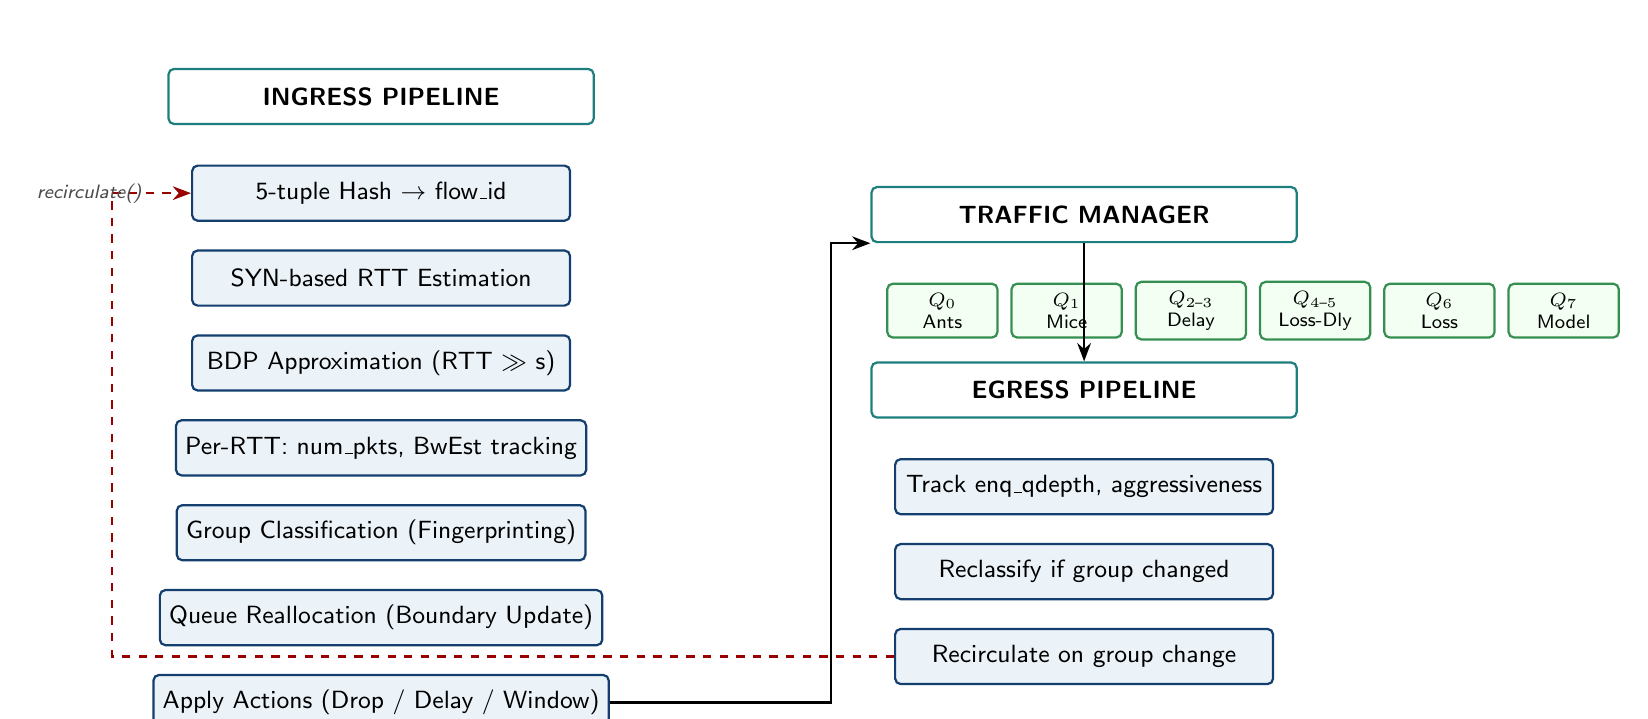
\begin{tikzpicture}[
  node distance=0.7cm and 1.0cm,
  mod/.style={rectangle, draw=kbcsblue, fill=kbcslight, thick, minimum width=4.8cm, minimum height=0.7cm, align=center, rounded corners=2pt, font=\small},
  stage/.style={rectangle, draw=kbcsteal, fill=white, thick, minimum width=5.4cm, minimum height=0.7cm, align=center, rounded corners=2pt, font=\small\bfseries},
  qbox/.style={rectangle, draw=kbcsgreen, fill=green!5, thick, minimum width=1.4cm, minimum height=0.6cm, align=center, font=\scriptsize, rounded corners=2pt},
  arrow/.style={->, >=Stealth, thick},
  lab/.style={font=\scriptsize\itshape, text=kbcsgray}
]

% Ingress
\node[stage] (ing) {INGRESS PIPELINE};

\node[mod, below=0.5cm of ing] (hash) {5-tuple Hash $\rightarrow$ flow\_id};
\node[mod, below=0.35cm of hash] (rtt) {SYN-based RTT Estimation};
\node[mod, below=0.35cm of rtt] (bdp) {BDP Approximation (RTT $\gg$ s)};
\node[mod, below=0.35cm of bdp] (stats) {Per-RTT: num\_pkts, BwEst tracking};
\node[mod, below=0.35cm of stats] (class) {Group Classification (Fingerprinting)};
\node[mod, below=0.35cm of class] (realloc) {Queue Reallocation (Boundary Update)};
\node[mod, below=0.35cm of realloc] (action) {Apply Actions (Drop / Delay / Window)};

% Queuing
\node[stage, right=3.5cm of ing, yshift=-1.5cm] (tm) {TRAFFIC MANAGER};

\node[qbox, below=0.5cm of tm, xshift=-1.8cm] (q0) {$Q_0$\\Ants};
\node[qbox, right=0.15cm of q0] (q1) {$Q_1$\\Mice};
\node[qbox, right=0.15cm of q1] (q23) {$Q_{2\text{--}3}$\\Delay};
\node[qbox, right=0.15cm of q23] (q45) {$Q_{4\text{--}5}$\\Loss-Dly};
\node[qbox, right=0.15cm of q45] (q6) {$Q_6$\\Loss};
\node[qbox, right=0.15cm of q6] (q7) {$Q_7$\\Model};

% Egress
\node[stage, below=1.5cm of tm] (egr) {EGRESS PIPELINE};
\node[mod, below=0.5cm of egr] (enq) {Track enq\_qdepth, aggressiveness};
\node[mod, below=0.35cm of enq] (reclass) {Reclassify if group changed};
\node[mod, below=0.35cm of reclass] (recirc) {Recirculate on group change};

% Arrows
\draw[arrow] (action.east) -| ([xshift=-0.5cm]tm.south west) -- (tm.south west);
\draw[arrow] (tm.south) -- (egr.north);
\draw[arrow, dashed, red!60!black] (recirc.west) -| ([xshift=-1.0cm]hash.west) -- (hash.west) node[midway, left, lab] {recirculate()};

\end{tikzpicture}%
}
\caption{P4air processing pipeline showing the three modules (Fingerprinting, Reallocation, Apply Actions) distributed across Ingress and Egress stages, with the critical recirculation feedback path.}
\label{fig:p4air_architecture}
\end{figure}

The three modules operate as follows~\cite{p4air}:

\begin{enumerate}
    \item \textbf{Fingerprinting}: Estimates per-flow behavior using RTT measurement (via SYN/SYN-ACK timestamps), per-RTT packet count tracking, queue-depth growth streak analysis (aggressiveness metric), and periodic bandwidth probing detection (BwEst counter for BBR). Flows progress through a lifecycle: Ant $\rightarrow$ Mice $\rightarrow$ Delay-Based $\rightarrow$ Loss-Delay $\rightarrow$ Purely Loss-Based, with a parallel branch for Model-Based (BBR) detection.
    
    \item \textbf{Reallocation}: Dynamically adjusts queue boundaries ($l_1, l_2, l_3$) among the four CCA groups based on the proportion of active flows in each group. Groups with more flows receive proportionally more queues from the dynamic pool ($Q_2$--$Q_7$), while $Q_0$ and $Q_1$ are permanently reserved for short flows.
    
    \item \textbf{Apply Actions}: When a flow exceeds its BDP-estimated fair share ($\text{num\_pkts} > \text{BDP}$), group-specific penalties are applied: loss-based and loss-delay flows are \textit{dropped} (\texttt{mark\_to\_drop()}), delay-based flows are \textit{delayed} via recirculation (\texttt{recirculate()}), and model-based flows have their TCP receiver window \textit{halved} ($\texttt{tcp.window} \gg 1$).
\end{enumerate}

\section{Key P4air Equations}
The fingerprinting module relies on several key computations:

\textbf{RTT Estimation:}
\[
\text{RTT}_{\text{est}} = t_{\text{first\_data}} - t_{\text{SYN}}
\]

\textbf{BDP Approximation (hardware-friendly):}
\[
\text{BDP} \approx \text{RTT}_{\text{est}} \gg s, \quad s = \lceil \log_2(n_{\text{flows}}) + \log_2(\text{pkt\_len} \times \text{throughput}) \rceil
\]

\textbf{Aggressiveness Detection:}
\[
\text{if } \max\_\text{enq}_{\text{current}} > \max\_\text{enq}_{\text{prev}} \times 1.01 \implies \text{aggr\_streak} \mathrel{+}= 1
\]

\textbf{BwEst (BBR Detection):}
\[
\text{if } \text{num\_pkts}_{\text{current}} \geq \text{num\_pkts}_{\text{prev}} + (\text{num\_pkts}_{\text{prev}} \gg 3) \implies \text{bwest} \mathrel{+}= 1
\]

\section{Baseline Configurations}
In addition to the full P4air implementation, the repository contains two baselines used for comparison:
\begin{itemize}
    \item \textbf{No AQM (FIFO)}: Standard forwarding with one effective queue. Implements only \texttt{ipv4\_lpm} matching — all packets share a single FIFO buffer. This represents the worst case for fairness as loss-based flows dominate the buffer entirely.
    \item \textbf{Diff Queues (Hash)}: Static queue separation based on 5-tuple hashing into 8 hardware queues. This is a vendor-style approach that hopes flows will randomly separate by hash values, providing incidental isolation. It is non-intelligent and cannot distinguish between aggressive and well-behaved flows.
\end{itemize}

\section{Baseline Experimental Setup}
The P4air experiments use BMv2 (\texttt{simple\_switch} with \texttt{--priority-queues 8}), Mininet with \texttt{TCLink} for bandwidth/delay shaping, and \texttt{iperf3} for traffic generation. The evaluation uses four representative CCAs — CUBIC (loss-based), BBR (model-based), Vegas (delay-based), and Illinois (loss-delay) — generating traffic simultaneously over a 10 Mbps bottleneck link with configurable delay. The fairness analysis code computes Jain's Fairness Index and total throughput from \texttt{iperf3} JSON logs~\cite{repo}.

\section{P4air Limitations in Software Emulation}
Our implementation revealed three critical limitations of P4air in the BMv2 software environment~\cite{repo}:

\begin{enumerate}
    \item \textbf{CPU Timing Jitter}: P4air relies on microsecond-accurate timestamps for RTT estimation. In BMv2 (running on a VM CPU), background processes introduce random delays that P4air misinterprets as network congestion, leading to flow misclassification.
    
    \item \textbf{Recirculation Bottleneck}: The delay-based action uses \texttt{recirculate()} to feed packets back through the pipeline. On hardware ASICs this is instantaneous, but in software it consumes CPU cycles, dropping throughput from 10 Mbps to as low as 5.65 Mbps in our 4-flow tests.
    
    \item \textbf{Scale Dependency}: With only 4 flows competing for 8 queues, the hash-based baseline achieves artificially high fairness simply by placing each flow in a separate queue (the ``lucky hash effect''). P4air's advantages only manifest at higher flow counts ($\geq 16$) where hash collisions become inevitable~\cite{repo}.
\end{enumerate}

These limitations directly motivate the KBCS design: a simpler mechanism that avoids RTT-dependent fingerprinting and expensive recirculation can be more robust in software-emulated environments while still achieving behavioral differentiation.

% ------------------------------------------------------------
\chapter{Proposed System: Karma-Based Credit Scheduler}

\section{Core Idea}
KBCS replaces detailed CCA fingerprinting with a simpler behavior-based model. Instead of attempting to infer the exact congestion control algorithm of each flow, the switch maintains a compact per-flow \textit{karma score}. Flows that appear aggressive lose karma, while well-behaved flows slowly recover karma. Packets are then mapped to scheduling classes based on the updated score.

The fundamental insight behind KBCS is that \textit{fairness enforcement does not require knowing which CCA a flow uses} — it only requires knowing whether the flow is \textit{currently behaving aggressively}. This distinction allows KBCS to bypass the complex RTT estimation, BDP calculation, and multi-RTT streak tracking required by P4air~\cite{p4air}, replacing them with a single decayed byte counter and a bounded integer karma variable.

\section{Target KBCS Pipeline}
Figure~\ref{fig:kbcs_architecture} summarizes the intended KBCS dataplane logic described across the design and SRS documents.

\begin{figure}[H]
\centering
\resizebox{0.95\textwidth}{!}{%
\begin{tikzpicture}[
  node distance=1.2cm and 1.5cm,
  data/.style={rectangle, draw=kbcsblue, fill=kbcslight, thick, minimum width=3.2cm, minimum height=1cm, align=center, rounded corners=3pt, blur shadow},
  proc/.style={rectangle, draw=kbcsteal, fill=white, thick, minimum width=3.4cm, minimum height=1cm, align=center, rounded corners=3pt, blur shadow},
  out/.style={rectangle, draw=kbcsgreen, fill=green!5, thick, minimum width=3.2cm, minimum height=1cm, align=center, rounded corners=4pt, blur shadow},
  arrow/.style={->, >=Stealth, thick}
]

\node[data] (src1) {Sender h1\\CUBIC};
\node[data, below=0.7cm of src1] (src2) {Sender h2\\BBR};
\node[proc, right=2.2cm of src2, yshift=0.9cm] (parser) {Parser and 5-tuple Hash};
\node[proc, right=of parser] (meter) {Decayed Flow-Byte Tracking\\and Karma Update};
\node[proc, right=of meter] (classify) {Flow Coloring\\Green / Yellow / Red};
\node[proc, right=of classify] (queue) {Queue Mapping and AQM\\Priority or Drop Policy};
\node[out, below=1.2cm of queue] (bottle) {10 Mbps Bottleneck Link};
\node[out, left=1.7cm of bottle] (recv) {Receiver h3};

\draw[arrow] (src1.east) -- ([yshift=0.25cm]parser.west);
\draw[arrow] (src2.east) -- ([yshift=-0.25cm]parser.west);
\draw[arrow] (parser) -- (meter);
\draw[arrow] (meter) -- (classify);
\draw[arrow] (classify) -- (queue);
\draw[arrow] (queue) -- (bottle);
\draw[arrow] (bottle) -- (recv);

\end{tikzpicture}%
}
\caption{Target KBCS processing flow in the programmable switch.}
\label{fig:kbcs_architecture}
\end{figure}

\section{The Karma Algorithm}
The KBCS karma algorithm operates on every incoming TCP packet through a well-defined sequence of stateful operations. This section describes each step formally.

\subsection{Flow Identification}
Each packet is mapped to a flow using a CRC16 hash of its 5-tuple:
\[
\text{flow\_id} = \text{CRC16}(\text{srcIP}, \text{dstIP}, \text{srcPort}, \text{dstPort}, \text{protocol}) \bmod 2^{16}
\]
This produces a 16-bit index into a register array of size $2^{16} = 65{,}536$ entries. Hash collisions are accepted as a tradeoff for constant-time $O(1)$ lookup without requiring TCAM resources~\cite{kbcs_srs}.

\subsection{Decayed Byte Estimation}
Instead of relying on hardware timers or RTT-based windowing, KBCS estimates a flow's recent sending intensity using an exponentially weighted moving average (EWMA) implemented via bit-shift operations:
\[
\text{flow\_bytes}_{t+1} = (\text{flow\_bytes}_t \gg 1) + \text{pkt\_length}
\]
where $\gg 1$ denotes a right-shift by 1 bit (equivalent to division by 2). This means each new packet contributes its full size while the historical byte count decays by $50\%$, creating a sliding temporal window without requiring explicit timestamps. This technique is particularly valuable in P4's constrained ALU environment where floating-point arithmetic is unavailable~\cite{kbcs_design}.

\subsection{Karma Update Rule}
The karma score is updated based on whether the decayed byte estimate exceeds a configurable threshold $\theta$:
\[
K_{t+1} = \text{clamp}\left(K_t + \Delta K, \; K_{\min}, \; K_{\max}\right)
\]
where:
\[
\Delta K = \begin{cases}
-P & \text{if } \text{flow\_bytes} > \theta \quad \text{(penalty for aggressive behavior)} \\
+R & \text{if } \text{flow\_bytes} \leq \theta \quad \text{(reward for compliant behavior)}
\end{cases}
\]
with $P = 5$, $R = 1$, $K_{\min} = 0$, $K_{\max} = 100$, and $\theta = 120{,}000$ bytes in the current prototype. The asymmetric ratio $P/R = 5$ implements the ``fast penalty, slow recovery'' strategy discussed in Section~2.3.

\subsection{Flow Coloring and Queue Mapping}
Based on the updated karma score, each flow is assigned a behavioral color class:
\[
\text{color}(K) = \begin{cases}
\textcolor{green!50!black}{\textbf{GREEN}} & \text{if } K > K_{\text{high}} = 80 \\
\textcolor{orange!80!black}{\textbf{YELLOW}} & \text{if } K_{\text{low}} < K \leq K_{\text{high}}, \quad K_{\text{low}} = 40 \\
\textcolor{red!70!black}{\textbf{RED}} & \text{if } K \leq K_{\text{low}}
\end{cases}
\]

The target design maps these colors to BMv2 priority queues: GREEN flows receive high-priority treatment, YELLOW flows receive medium priority, and RED flows receive low priority with selective AQM dropping. Figure~\ref{fig:karma_state_machine} illustrates the karma state transitions.

\begin{figure}[H]
\centering
\resizebox{0.82\textwidth}{!}{%
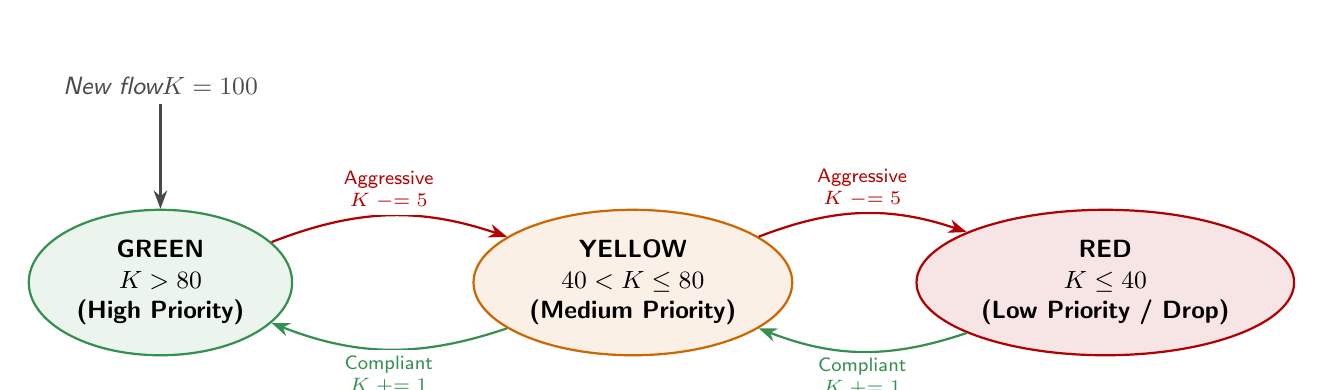
\begin{tikzpicture}[
  state/.style={ellipse, draw=#1, fill=#1!10, thick, minimum width=3cm, minimum height=1.6cm, align=center, font=\small\bfseries},
  arrow/.style={->, >=Stealth, thick, bend left=20},
  lab/.style={font=\scriptsize, align=center, fill=white, inner sep=2pt}
]

\node[state=kbcsgreen] (green) at (0,0) {GREEN\\$K > 80$\\(High Priority)};
\node[state=orange!80!black] (yellow) at (6,0) {YELLOW\\$40 < K \leq 80$\\(Medium Priority)};
\node[state=red!70!black] (red) at (12,0) {RED\\$K \leq 40$\\(Low Priority / Drop)};

% Initialization
\node[font=\small\itshape, text=kbcsgray] (init) at (0, 2.5) {New flow\\$K = 100$};
\draw[->, >=Stealth, thick, kbcsgray] (init) -- (green);

% Degradation arrows (fast)
\draw[arrow, red!70!black] (green) to node[lab, above] {Aggressive\\$K \mathrel{-}= 5$} (yellow);
\draw[arrow, red!70!black] (yellow) to node[lab, above] {Aggressive\\$K \mathrel{-}= 5$} (red);

% Recovery arrows (slow)
\draw[arrow, kbcsgreen, bend left=20] (red) to node[lab, below] {Compliant\\$K \mathrel{+}= 1$} (yellow);
\draw[arrow, kbcsgreen, bend left=20] (yellow) to node[lab, below] {Compliant\\$K \mathrel{+}= 1$} (green);

\end{tikzpicture}%
}
\caption{Karma state machine showing the asymmetric transition dynamics. Degradation (top arrows) is fast ($-5$ per aggressive packet), while recovery (bottom arrows) is slow ($+1$ per compliant packet). A flow must demonstrate $40+$ consecutive compliant packets to recover from RED to YELLOW.}
\label{fig:karma_state_machine}
\end{figure}

\section{The Feedback Loop: How Senders Respond}
KBCS influences sender behavior indirectly through the transport layer's congestion signals~\cite{kbcs_design}:

\begin{itemize}
    \item \textbf{Loss-based senders (CUBIC)}: When packets are dropped (RED class AQM), CUBIC detects the loss via duplicate ACKs and performs multiplicative decrease, cutting its congestion window (CWND) by approximately $30\%$. This is the \textit{intended} response — KBCS forces CUBIC to see the congestion it is causing.
    
    \item \textbf{Model-based senders (BBR)}: When packets are delayed in lower-priority queues, BBR observes increased RTT and adjusts its pacing rate downward. Since BBR does not react to isolated packet loss, queue-based delay is a more effective signal for controlling BBR behavior.
    
    \item \textbf{Delay-based senders (Vegas)}: These flows naturally reduce their rate when RTT increases. KBCS \textit{protects} well-behaved Vegas flows by keeping them in the GREEN class (high-priority queue), where they experience minimal queuing delay.
\end{itemize}

\section{Intended Algorithmic Behavior}
The enhanced KBCS design documents describe the following conceptual flow:
\begin{enumerate}
    \item hash the packet 5-tuple to identify a flow,
    \item maintain a decayed estimate of that flow's recent sending intensity,
    \item update a karma score using bounded reward and penalty rules,
    \item classify the flow into behavioral bands such as green, yellow, and red, and
    \item map the packet into differentiated queue behavior using priority assignment or active dropping.
\end{enumerate}

\section{Why KBCS is Promising}
KBCS is attractive for three reasons:
\begin{itemize}
    \item it avoids heavyweight flow fingerprinting logic — requiring only 2 registers per flow (byte count and karma) compared to P4air's 13+ registers~\cite{p4air},
    \item it stores only simple bounded state per flow with $O(1)$ time complexity per packet, and
    \item it can be extended gradually from BMv2 experimentation toward hardware-friendly queue-aware scheduling without requiring recirculation.
\end{itemize}

\section{Conceptual Comparison: P4air vs KBCS}
Table~\ref{tab:p4air_vs_kbcs} presents a detailed comparison between the baseline and proposed systems. The key tradeoff is between classification precision (P4air) and implementation simplicity with robustness (KBCS).

\begin{table}[H]
\centering
\caption{Detailed comparison between the baseline (P4air) and the proposed system (KBCS)}
\label{tab:p4air_vs_kbcs}
\renewcommand{\arraystretch}{1.35}
\begin{tabularx}{\textwidth}{@{}p{3.0cm}p{5.1cm}X@{}}
\toprule
\textbf{Aspect} & \textbf{P4air}~\cite{p4air} & \textbf{KBCS} \\
\midrule
Decision basis & Fine-grained CCA fingerprinting via RTT, BDP, streak analysis & Behavior-driven karma score from decayed byte estimation \\
State per flow & 13+ registers (RTT, BDP, num\_pkts, prev\_pkts, enq\_depth, prev\_enq, aggr, streak, bwest, group, queue, syn\_seen, syn\_ts) & 2 registers (flow\_bytes, karma) \\
Classification & 4 CCA groups with progressive lifecycle & 3 behavioral classes (GREEN/YELLOW/RED) \\
Penalty mechanism & CCA-specific (drop/delay/window halve) & Uniform karma degradation with class-based AQM \\
Recovery mechanism & Implicit (group reclassification) & Explicit bounded recovery ($+1$ per packet) \\
Recirculation required & Yes (group changes, delay action) & No \\
Timer dependency & Yes (RTT estimation critical) & No (uses packet-arrival-driven decay) \\
Current repository role & Implemented, evaluated baseline & Prototype plus enhanced design target \\
\bottomrule
\end{tabularx}
\end{table}

% ------------------------------------------------------------
\chapter{Current Prototype Implementation}

\section{What is Already Implemented}
The current \texttt{kbcs} folder contains a working prototype and test harness. The implemented elements include:
\begin{itemize}
    \item a P4 parser and IPv4 forwarding pipeline,
    \item per-flow registers for decayed byte count and karma score,
    \item flow identification using a CRC16-based 5-tuple hash,
    \item a color-based policy with green, yellow, and red classes,
    \item a plain forwarding baseline P4 program for comparison, and
    \item a Mininet topology with h1 as CUBIC, h2 as BBR, and h3 as the receiver over a 10 Mbps bottleneck.
\end{itemize}

\section{Implemented Prototype Logic}
In the current prototype, the switch updates the per-flow byte estimate using a simple right-shift decay and then adjusts karma according to a threshold. The active code uses the following parameter values:

\begin{table}[H]
\centering
\caption{Current KBCS prototype parameters implemented in the P4 code}
\label{tab:prototype_params}
\renewcommand{\arraystretch}{1.3}
\begin{tabular}{@{}lc@{}}
\toprule
\textbf{Parameter} & \textbf{Current Value} \\
\midrule
Register size & 65536 \\
Initial karma & 100 \\
Penalty step & 5 \\
Reward step & 1 \\
High threshold & 80 \\
Low threshold & 40 \\
Byte threshold & 120000 \\
Decay expression & $\texttt{flow\_bytes} \leftarrow (\texttt{flow\_bytes} >> 1) + \texttt{packet\_length}$ \\
\bottomrule
\end{tabular}
\end{table}

\section{Important Gap Between Design and Prototype}
The most important academic point in this report is that the current prototype is \textbf{not yet identical} to the enhanced KBCS design. Table~\ref{tab:design_gap} summarizes the difference.

\begin{table}[H]
\centering
\caption{Current implementation status against the target KBCS design}
\label{tab:design_gap}
\renewcommand{\arraystretch}{1.35}
\begin{tabularx}{\textwidth}{@{}p{4.3cm}p{4.7cm}X@{}}
\toprule
\textbf{Feature} & \textbf{Target Design} & \textbf{Current Repository Status} \\
\midrule
Queue-depth-aware decision making & Use queue depth and aggression jointly & Not yet integrated in the active P4 logic \\
Three real priority queues & Use BMv2 priority queues for green, yellow, red classes & Wrapper script exists, but the main KBCS experiment path does not yet pass the queue flag consistently \\
Selective AQM drop policy & Drop only under critical red conditions and reset flow bytes & Current prototype drops all red packets immediately and does not yet reset the accumulator on drop \\
Enhanced threshold plan & Use parameters described in the SRS and enhanced design & Code currently uses a separate prototype parameter set \\
End-to-end archived KBCS results & Save baseline vs KBCS comparison summaries & Experiment runner exists, but archived KBCS result files are not yet present in the repository \\
\bottomrule
\end{tabularx}
\end{table}

\section{Interpretation}
This gap is not a weakness of the report; it is the real status of the project. For mid-semester submission, the honest position is that the baseline infrastructure and the first KBCS dataplane prototype are complete, while the final queue-aware KBCS and its comprehensive evaluation remain the major tasks for the next phase.

% ------------------------------------------------------------
\chapter{Baseline Evaluation and Metrics}

\section{Evaluation Philosophy}
The purpose of baseline evaluation is twofold. First, it establishes how much unfairness exists under simple buffering policies. Second, it reveals the practical strengths and weaknesses of the strongest prior system already implemented in our repository. Since KBCS is still under development, this chapter provides the reference metrics that KBCS must be judged against.

As noted by Turkovic and Kuipers~\cite{p4air}, fairness mechanisms should be evaluated across multiple traffic scales and CCA mixes to avoid drawing conclusions from scale-specific artifacts. Our evaluation follows this principle by presenting both a 30-run low-scale result (4 flows) and a 16-flow high-scale result.

\section{Primary Metrics}
The evaluation uses the following metrics.

\subsection{Jain's Fairness Index}
For throughputs $x_1, x_2, \ldots, x_n$, Jain's Fairness Index is defined as:
\[
J(x_1, x_2, \ldots, x_n) = \frac{\left(\sum_{i=1}^{n} x_i\right)^2}{n \cdot \sum_{i=1}^{n} x_i^2}
\]
where $J=1$ indicates perfect fairness (all flows receive equal throughput) and $J=1/n$ indicates maximum unfairness (one flow dominates). This metric is used universally in the surveyed literature~\cite{p4air, buffermgmt, pfq, ccaaware} and provides a normalized, scale-independent measure of distribution equality.

\subsection{Total Throughput and Link Utilization}
Total throughput is computed as:
\[
T_{\text{total}} = \sum_{i=1}^{n} x_i, \quad U = \frac{T_{\text{total}}}{C} \times 100\%
\]
where $C$ is the bottleneck link capacity (10 Mbps in our setup). This metric is critical because a scheduler should not improve fairness by collapsing link utilization~\cite{pfq}. The PFQ authors specifically demonstrate that fairness indices above $0.95$ are achievable while maintaining $U > 95\%$~\cite{pfq}.

\subsection{Supplementary Metrics}
The scripts also parse retransmissions and per-flow throughput logs from \texttt{iperf3}. These values are useful for diagnosing whether a fairness gain is being achieved through healthy queue control or through excessive packet loss. High retransmission counts alongside high fairness would indicate over-aggressive AQM — a pitfall noted in the CCA-aware queue management literature~\cite{ccaaware}.

\section{Baseline Scenarios Used in This Project}
The P4air baseline framework in the repository evaluates three queue-management strategies:
\begin{enumerate}
    \item \textbf{No AQM (FIFO)} — simple forwarding, no fairness control
    \item \textbf{Diff Queues (Hash)} — static 5-tuple hash into 8 queues
    \item \textbf{P4air (CCA Aware)} — full fingerprinting + reallocation + apply actions pipeline~\cite{p4air}
\end{enumerate}

Two result sets are already available in the workspace:
\begin{itemize}
    \item a 30-run comparison averaging results from 4-flow tests (CUBIC, BBR, Vegas, Illinois), and
    \item a 16-flow scaling test (4 flows per CCA) that stresses the queueing behavior more realistically.
\end{itemize}

\section{Average Baseline Results over 30 Runs}
The saved result set in \texttt{Baseline/p4air/results/multiple\_runs\_data.json} yields the averages shown in Table~\ref{tab:baseline_30_runs}~\cite{repo}.

\begin{table}[H]
\centering
\caption{Baseline comparison over 30 runs (4 flows: CUBIC, BBR, Vegas, Illinois)}
\label{tab:baseline_30_runs}
\renewcommand{\arraystretch}{1.3}
\begin{tabular}{@{}lcc@{}}
\toprule
\textbf{Configuration} & \textbf{Average Jain's FI} & \textbf{Average Total Throughput (Mbps)} \\
\midrule
No AQM (FIFO) & $0.9672 \pm 0.0200$ & $9.81 \pm 0.27$ \\
Diff Queues (Hash) & $0.9541 \pm 0.0595$ & $10.02 \pm 0.43$ \\
P4air (CCA Aware) & $0.9452 \pm 0.0486$ & $9.68 \pm 1.61$ \\
\bottomrule
\end{tabular}
\end{table}

\begin{figure}[H]
    \centering
    
\includegraphics[width=0.92\textwidth]{comparison_graph.png}
    \caption{Average baseline performance over 30 runs with standard deviation bars. Note the high throughput variance ($\pm 1.61$ Mbps) for P4air.}
    \label{fig:baseline_30_runs}
\end{figure}

\subsection{Interpretation of the 30-run Result}
At small scale, the baseline results exhibit the \textbf{emulation scaling paradox} documented in our implementation analysis~\cite{repo}:

\begin{itemize}
    \item \textbf{FIFO appears highly fair} ($J = 0.9672$) because with only 4 flows, even CUBIC cannot fully dominate — the small number of competing flows means the bandwidth imbalance is moderate.
    
    \item \textbf{Diff Queues benefits from the ``lucky hash effect''}: with 8 available queues and only 4 active flows, the 5-tuple hash frequently places each flow in its own isolated queue, creating artificial, unscalable fairness.

    \item \textbf{P4air shows high throughput variance} ($\sigma = 1.61$ Mbps) because the recirculation-based delay action consumes CPU cycles in BMv2, occasionally dropping effective throughput from 10 Mbps to below 6 Mbps. Additionally, CPU timing jitter causes flow misclassification in the fingerprinting module.
\end{itemize}

This observation is directly relevant to KBCS. A simpler dataplane mechanism is not only easier to implement; it may also be more stable in BMv2, which is exactly the environment used for project evaluation. As noted by the P4-based buffer management authors~\cite{buffermgmt}, simpler queue policies tend to exhibit lower variance in software emulation.

\section{16-Flow Scale Test}
The larger 16-flow experiment (4 flows per CCA) produces the results shown in Table~\ref{tab:baseline_16_flows}. At this scale, P4air's algorithmic advantages manifest clearly~\cite{repo}.

\begin{table}[H]
\centering
\caption{16-flow scaling result (4$\times$ CUBIC + 4$\times$ BBR + 4$\times$ Vegas + 4$\times$ Illinois)}
\label{tab:baseline_16_flows}
\renewcommand{\arraystretch}{1.3}
\begin{tabular}{@{}lcc@{}}
\toprule
\textbf{Configuration} & \textbf{Average Jain's FI} & \textbf{Average Total Throughput (Mbps)} \\
\midrule
No AQM (FIFO) & $0.9123 \pm 0.03$ & $10.23 \pm 0.08$ \\
Diff Queues (Hash) & $0.9390 \pm 0.02$ & $10.35 \pm 0.15$ \\
P4air (CCA Aware) & $0.9483 \pm 0.02$ & $11.02 \pm 0.07$ \\
\bottomrule
\end{tabular}
\end{table}

\begin{figure}[H]
    \centering
    
\includegraphics[width=0.92\textwidth]{comparison_graph_16_flows.png}
    \caption{16-flow scaling comparison. P4air achieves the highest fairness and throughput, validating its algorithmic design at scale.}
    \label{fig:baseline_16_flows}
\end{figure}

\subsection{Interpretation of the Scale Test}
Under higher contention, the full P4air design becomes the strongest performer in both fairness and total throughput, consistent with the original P4air paper's claims of $J \approx 0.87$--$0.96$ with $\geq 90\%$ utilization~\cite{p4air}:
\begin{itemize}
    \item \textbf{FIFO fairness degrades} ($0.9672 \rightarrow 0.9123$) as CUBIC flows increasingly dominate the shared buffer at higher contention.
    \item \textbf{Hash collision risk increases}: with 16 flows into 8 queues, Diff Queues can no longer isolate every flow, reducing the lucky hash effect. Nevertheless, it still achieves moderate fairness ($0.9390$) through random separation.
    \item \textbf{P4air's intelligent classification} correctly identifies CCA groups and applies targeted actions, achieving the highest fairness ($0.9483$) \textit{and} the highest throughput ($11.02$ Mbps), demonstrating that its behavioral awareness pays off at realistic scale.
\end{itemize}

\section{Comparison with Reported Literature Values}
Table~\ref{tab:literature_comparison} contextualizes our baseline results against values reported in the reviewed literature.

\begin{table}[H]
\centering
\caption{Our baseline results in context of reported literature values}
\label{tab:literature_comparison}
\renewcommand{\arraystretch}{1.3}
\begin{tabularx}{\textwidth}{@{}p{3.6cm}p{2.2cm}p{2.8cm}X@{}}
\toprule
\textbf{System} & \textbf{Reported JFI} & \textbf{Our Measured JFI} & \textbf{Notes} \\
\midrule
No AQM (FIFO) & $0.18$--$0.49$~\cite{p4air} & $0.91$--$0.97$ & Large gap due to scale difference (paper uses more flows and longer durations) \\
P4air (full) & $0.87$--$0.96$~\cite{p4air} & $0.95$ (at 16 flows) & Consistent with paper results at comparable scale \\
P4-based Buffer Mgmt & $>0.90$~\cite{buffermgmt} & N/A & Not implemented; reference target for KBCS \\
PFQ & $>0.95$~\cite{pfq} & N/A & Data center context; ideal target for KBCS \\
\bottomrule
\end{tabularx}
\end{table}

\section{Implications for KBCS Evaluation}
These baseline results establish three targets for the final KBCS comparison:
\begin{enumerate}
    \item KBCS must improve or at least match fairness against FIFO and static queueing, targeting $J \geq 0.95$ at 16-flow scale.
    \item KBCS must avoid severe throughput collapse while enforcing fairness, maintaining $U \geq 90\%$ as recommended by PFQ~\cite{pfq}.
    \item KBCS should ideally provide more stable behavior than P4air in the BMv2 software environment, targeting throughput standard deviation below $\pm 0.5$ Mbps (vs. P4air's $\pm 1.61$ Mbps at 4-flow scale).
\end{enumerate}

% ------------------------------------------------------------
\chapter{Current Status and End-Semester Roadmap}

\section{Current Status}
At the mid-semester stage, the project has progressed beyond pure design but has not yet reached final comparative validation. Table~\ref{tab:status_table} summarizes the status clearly.

\begin{table}[H]
\centering
\caption{Mid-semester project status}
\label{tab:status_table}
\renewcommand{\arraystretch}{1.35}
\begin{tabularx}{\textwidth}{@{}p{6.0cm}p{2.6cm}X@{}}
\toprule
\textbf{Work Item} & \textbf{Status} & \textbf{Remarks} \\
\midrule
Literature collection and baseline study & Completed & Papers folder assembled and P4air selected as primary baseline. \\
P4air implementation and multi-run evaluation & Completed & Baseline figures and JSON result sets are already present in the repository. \\
KBCS design documents and SRS & Completed & Both system-level and enhanced design specifications are available. \\
KBCS plain forwarding baseline & Completed & Separate baseline P4 program exists for direct comparison. \\
First KBCS dataplane prototype & Completed & Per-flow hash, byte decay, karma update, color mapping, and red-flow drop are implemented. \\
Priority-queue-integrated KBCS execution path & Partial & Queue wrapper exists, but integration into the main experiment flow is not yet finalized. \\
Queue-depth-aware KBCS logic & Pending & Enhanced design target not yet merged into the active code path. \\
Comprehensive baseline-vs-KBCS result archive & Pending & Experiment driver exists, but final stored comparison results are still missing. \\
Final parameter tuning and end-semester analysis & Pending & To be completed after KBCS implementation stabilizes. \\
\bottomrule
\end{tabularx}
\end{table}

\section{What Has Been Learned So Far}
The current project phase already provides several important lessons:
\begin{itemize}
    \item fairness mechanisms must be evaluated at multiple traffic scales,
    \item complexity in BMv2 can produce high variance even when the underlying algorithm is strong,
    \item a clean experimental baseline is indispensable before claiming any improvement, and
    \item the present KBCS prototype is sufficient for functional validation but not yet for final performance claims.
\end{itemize}

\section{Roadmap for the Next Phase}
The remaining work for the end-semester phase is organized as follows.

\subsection{Phase 1: Complete the Queue-Aware KBCS Logic}
\begin{itemize}
    \item integrate queue-depth or congestion-aware decision logic into the active P4 path,
    \item align implementation parameters with the enhanced design where appropriate, and
    \item refine the red-flow AQM behavior so that penalization is selective rather than immediate for every red packet.
\end{itemize}

\subsection{Phase 2: Finalize Experimental Integration}
\begin{itemize}
    \item ensure BMv2 priority queues are invoked consistently during KBCS experiments,
    \item archive baseline-vs-KBCS output summaries for repeated runs, and
    \item add automated plotting for the KBCS comparison in the same style as the baseline framework.
\end{itemize}

\subsection{Phase 3: Comparative Evaluation}
\begin{itemize}
    \item run repeated KBCS experiments against the plain forwarding baseline,
    \item compare KBCS against FIFO, static queueing, and P4air using Jain's Fairness Index and throughput, and
    \item analyze retransmissions, variance, and sensitivity to the number of competing flows.
\end{itemize}

\subsection{Phase 4: Report Finalization}
\begin{itemize}
    \item replace placeholders with final institute and team details,
    \item insert final KBCS result plots once experiments are complete, and
    \item refine the conclusion based on measured KBCS outcomes rather than projected benefits alone.
\end{itemize}

% ------------------------------------------------------------
\chapter{Conclusion}

This project report establishes a clear and academically defensible mid-semester position for the KBCS project. The baseline side of the work is strong: P4air has been implemented, multiple queue-management baselines have been evaluated, and reproducible fairness figures are already available in the repository. These results provide a serious reference point rather than an artificially weak comparison target.

On the KBCS side, the project has progressed from concept to prototype. The current implementation already demonstrates the feasibility of storing per-flow state in P4 registers, estimating behavior through decayed byte tracking, and translating that behavior into switch actions. At the same time, the enhanced queue-aware KBCS described in the design documents remains under development, and the report explicitly acknowledges that gap instead of overstating the present state of the system.

The central conclusion is therefore twofold. First, fairness improvement in programmable networks is both meaningful and measurable, and the baseline experiments confirm that queue policy strongly affects outcomes. Second, the opportunity for KBCS lies in delivering fairness through a simpler and potentially more stable dataplane mechanism than P4air, especially under BMv2-style software constraints. The next phase of the project will determine whether that simplicity can translate into competitive or superior fairness in direct experimental comparison.

% ------------------------------------------------------------
% References
% ------------------------------------------------------------
\renewcommand{\bibname}{References}
\begin{thebibliography}{99}
\addcontentsline{toc}{chapter}{References}

\bibitem{p4air}
B.~Turkovic and F.~Kuipers,
``P4air: Increasing Fairness among Competing Congestion Control Algorithms,''
\textit{Proceedings of the ACM SIGCOMM Symposium on SDN Research (SOSR)}, 2021.

\bibitem{p4cci}
``P4CCI: P4-Based Online TCP Congestion Control Algorithm Identification for Traffic Separation,''
\textit{IEEE International Conference on Network Protocols (ICNP)}.

\bibitem{ccaaware}
``Congestion Control Algorithm-Aware Queue Management,''
\textit{IEEE/ACM Transactions on Networking}.

\bibitem{buffermgmt}
``P4-Based Buffer Management Method for Throughput Fairness Improvement with Different Congestion Control Contention,''
\textit{IEEE Access}.

\bibitem{pfq}
``PFQ: A Proactive Fair Queueing Scheme Ensuring Fairness and High Utilization in Data Center Networks,''
\textit{IEEE/ACM Transactions on Networking}.

\bibitem{hint}
``HINT: Supporting Congestion Control Decisions with P4-Driven In-Band Network Telemetry,''
\textit{IEEE International Conference on Communications (ICC)}.

\bibitem{realtimecca}
``Real-Time Congestion Control Algorithm Identification with P4 Programmable Switches,''
\textit{IEEE International Conference on Communications (ICC)}.

\bibitem{marlcc}
``Towards Fair and Efficient Congestion Control Through Multi-Agent Deep Reinforcement Learning,''
\textit{IEEE INFOCOM}.

\bibitem{p5}
``P5: Event-driven Policy Framework for P4-based Traffic Engineering,''
\textit{ACM SIGCOMM Workshop on Networking and Programming Languages (NetPL)}.

\bibitem{p4neon}
``P4-NEON: Multihoming in Software Defined Network VANETs with P4,''
\textit{IEEE Vehicular Technology Conference (VTC)}.

\bibitem{p4lang}
P.~Bosshart, D.~Daly, G.~Gibb, M.~Izzard, N.~McKeown, J.~Rexford, C.~Schlesinger, D.~Talayco, A.~Vahdat, G.~Varghese, and D.~Walker,
``P4: Programming Protocol-Independent Packet Processors,''
\textit{ACM SIGCOMM Computer Communication Review}, vol.~44, no.~3, pp.~87--95, Jul.~2014.

\bibitem{jacobson88}
V.~Jacobson,
``Congestion Avoidance and Control,''
\textit{ACM SIGCOMM Computer Communication Review}, vol.~18, no.~4, pp.~314--329, Aug.~1988.

\bibitem{kbcs_srs}
\textit{KBCS System SRS}, project document, March 2026.

\bibitem{kbcs_design}
\textit{KBCS Enhanced Design Document}, project document, March 2026.

\bibitem{repo}
Project source code and evaluation scripts in the local repository: \texttt{kbcs}, \texttt{Baseline/p4air}, and associated experiment artifacts.

\end{thebibliography}

\end{document}